\section{Introduction of Real-time POV}

\begin{frame}{Previous Work}
	\begin{quote}
    	\Large
    	Hwang, Gwan-Hwan, Wei-Sian Huang, and Jenn-Zjone Peng. \textcolor{blue}{"Real-time proof of violation for cloud storage."} Cloud Computing Technology and Science (CloudCom), 2014 IEEE 6th International Conference on. IEEE, 2014.
	\end{quote}
\end{frame}

\begin{frame}{POV - Proof of Violation}
	定義以下三個 Tuples:
    ~\\
    ~\\
	\begin{itemize}  
        \item \textcolor{blue}{Properties}
	        \begin{itemize}
            	\item Data Integrity
                \item Write Serializability
                \item Read Freshness
            \end{itemize}
        \item \textcolor{blue}{A cryptographic accountability protocol (CAP)}
	        \begin{itemize}
            	\item 在 User 和 Service Provider 之間交換的訊息加上簽章,\\ 藉由此 Cryptographic Proof 讓雙方不可否認自己做過的事
            \end{itemize}
        \item \textcolor{blue}{Auditing}
            \begin{itemize}
            	\item 利用收集的 Cryptographic Proof 來證明是否違反 Properties
            \end{itemize}
    \end{itemize}
\end{frame}

\begin{frame}{Real-time Proof of Violation for Cloud Storage}
{2014 IEEE 6th International Conference on Cloud Computing Technology and Science}
	\begin{center}
		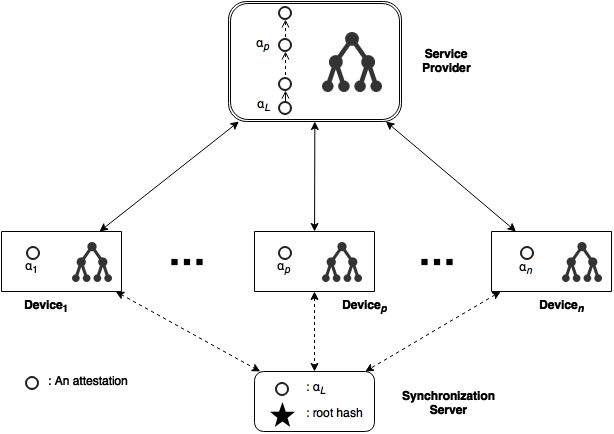
\includegraphics[height=.8\textheight]{wei_shian}
	\end{center}
\end{frame}

\begin{frame}{Merkle Tree}
	\begin{center}
		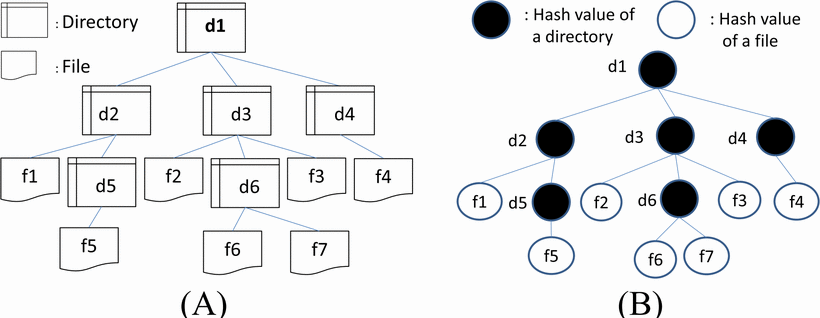
\includegraphics[width=\textwidth]{merkle_tree}
	\end{center}
\end{frame}

\begin{frame}{Real-time Proof of Violation for Cloud Storage}
{2014 IEEE 6th International Conference on Cloud Computing Technology and Science}
	\begin{center}
		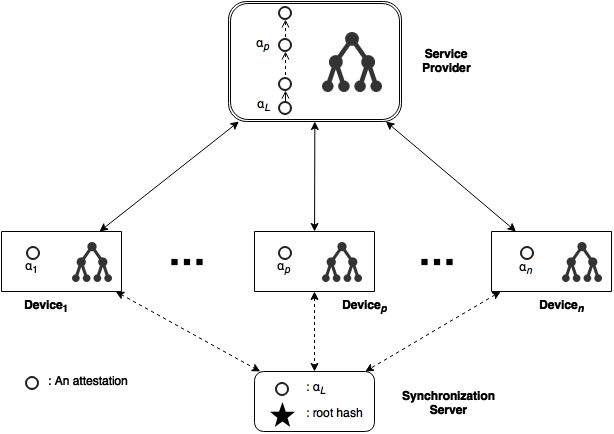
\includegraphics[height=.8\textheight]{wei_shian}
	\end{center}
\end{frame}

\begin{frame}{Worst-case}
	\textcolor{blue}{若有個 device 很久沒有使用,下次要上傳下載檔案前需要花很長的時間將 merkle tree 更新到最新\\
	累積的 hash chain 越長,使用者等待的時間越久}\\
	~\\
	~\\
	~\\
	\begin{center}
		\includegraphics[width=.5\textwidth]{worst_case}
	\end{center}
\end{frame}